% !TeX program = xelatex
% !TeX root = main.tex
\section{实证比较}
\sectionlead{section-4}{四、实证比较}{研究投入呈右偏长尾，均值难以代表典型投资者。异质性来自哪里？股票、投资者，还是交易时点。}

\begin{frame}[label=empirical-why]{为什么进一步比较股票、投资者与交易情境}
  \crumb{Part 4}{实证动机}{Tables 2--3 · V--VII}
  \small
  \begin{tabularx}{\linewidth}{@{}L{.29\linewidth}YL{.24\linewidth}@{}}
    \toprule 已见事实 & 需要进一步回答 & 分析方向\\\midrule
    价格图关注最常见，均值远高于中位数 & 哪些股票和主题吸引更多研究？ & 股票 \(\times\) 月\\\midrule
    交易笔数与每笔研究相关 \(-0.10\) & 交易频率，不足解释研究偏好 & 投资者（家庭）主题矩阵\\\midrule
    - & 研究和交易时点如何？ & 相对订单时点与路径\\\bottomrule
  \end{tabularx}\par\medskip
\end{frame}

\subsection{4.1 股票与投资者}
\begin{frame}[label=slices]{三种分析对象依次研究}
  \crumb{Part 4}{4.1 股票与投资者}{论文 V--VII}
  \small
  \begin{tabularx}{\linewidth}{@{}L{.24\linewidth}YY@{}}
    \toprule 一行是什么 & 字段示意 & 问题和方法\\\midrule
    股票 \(\times\) 月 & \(\underbrace{(j,m)}_{\text{股票、月份}}\ \mid\ \underbrace{A,L,D}_{\text{三项关注量}}\) &
      \textbf{关注分布}：前 1,000 大 CRSP 股票，月面板回归。\\\midrule
    投资者（家庭） & \(\underbrace{i}_{\text{投资者}}\ \mid\ \underbrace{B_{i1},\ldots,B_{i,13}}_{\text{各主题列}}\ \mid\ S_i\) &
      \textbf{研究风格}：研究的倾向，PCA主成分分析。\\\midrule
    投资者 \(\times\) 股票 \(\times\) 订单 &
      \((i,j,e)\) 投资者、股票、订单\newline \((\tau,k)\) 相对时点、主题 &
      \textbf{交易时序}：研究交易的路径。\\
    \bottomrule
  \end{tabularx}
  \finding{按股票、投资者和交易事件，逐步考察投资者行为的异质性。}
\end{frame}

\begin{frame}[t,label=design]{股票月回归区分广度、用时和内容}
  \crumb{Part 4}{4.1 股票与投资者 · 股票月规格}{Table 4}
  \vspace{-0.8em}
  \[
    Y_{jm}=\alpha+\beta z(\ln \mathrm{Cap}_{jm})+\gamma^\top Z_{jm}
               +\delta_{\mathrm{FF49}(j)}+\varepsilon_{jm},
    \qquad Y \in \{A,L,D\}.
  \]
  \small
  \begin{tabularx}{\linewidth}{@{}L{.25\linewidth}Y@{}}
    \toprule \(A\) 覆盖率 (1--3) & 月内研究过该股的投资者比例（百分点）。\\
    \(L\) 总用时 (4) & \(\ln(1+\text{研究该股票的时长})\)。\\
    \(D\) 内容倾斜 (5--6) & 查看价格图的比例，减查看基本面信息的比例。\\\bottomrule
  \end{tabularx}
  \medskip
  {\small \(j\)：股票；\(m\)：月份。(1) 只放市值；扩展规格加事件、股票特征及 FF49 行业项。}
  \finding{3,962 个股票月，原表 Newey--West 月度滞后 2 阶。三个被解释变量，\(A\) 和 \(L\) 对应关注广度与总投入，\(D\) 看主题构成。}
  \scriptsize\jump{appendix-2}{A2 · 回归全表}
\end{frame}

\begin{frame}[label=size-coefficients]{市值与研究覆盖率、总用时的关系}
  \crumb{Part 4}{4.1 股票与投资者 · 市值系数}{据 Table 4 (1)--(4) 重绘}
  \pair{\small\textbf{覆盖率 A · 百分点}\par
    \begin{tikzpicture}[x=2.25cm,y=.7cm,font=\small]
      \draw[quiet!40] (0,-.3)--(0,2.4);
      \foreach \y/\b/\t/\id in {2/1.03/14.42/{(1 仅对数市值)},1/1.33/13.57/{(2 市值＋股票特征、行业固定效应)},0/1.13/11.35/{(3 在(2)基础上，加散户交易特征)}} {
        \pgfmathsetmacro{\se}{1.96*\b/\t}
        \node[anchor=east] at (0,\y) {\id};
        \draw[sampleblue,thick] ({\b-\se},\y)--({\b+\se},\y);
        \fill[sampleblue] (\b,\y) circle[radius=1.7pt];
        \node[above,font=\scriptsize] at (\b,\y) {\b\;(\t)};}
      \foreach \x in {0,.5,1,1.5} \node[below] at (\x,-.3) {\pgfmathprintnumber{\x}};
    \end{tikzpicture}}
  {\small\textbf{总用时 L · 对数点}\par
    \begin{tikzpicture}[x=5.1cm,y=.7cm,font=\small]
      \draw[quiet!40] (0,-.3)--(0,2.4);
      \draw[sampleteal,thick] (.427,1)--(.553,1);
      \fill[sampleteal] (.49,1) circle[radius=1.7pt];
      \node[above,font=\scriptsize] at (.49,1) {0.49\;(15.23)};
      \node[anchor=east] at (0,1) {(4 完整的控制变量)};
      \foreach \x in {0,.2,.4,.6} \node[below] at (\x,-.3) {\pgfmathprintnumber{\x}};
    \end{tikzpicture}}
  \medskip
  {\small 连续解释变量增加 1 个标准差。点为系数，括号为 \(t值\)。}\par\medskip
  \finding{不同规格下，市值与研究覆盖率、总用时均显著正相关。}
\end{frame}

\begin{frame}[label=size]{仅市值解释约三成的覆盖率变异}
  \crumb{Part 4}{4.1 股票与投资者 · 解释度与量级}{Table 4 (1)--(4)}
  \pair{
    \textbf{覆盖率 \(R^2\)}\par
    \begin{tikzpicture}[x=6.85cm,y=.69cm,font=\small]
      \foreach \y/\r/\id in {2/.315/{(1)},1/.447/{(2)},0/.484/{(3)}} {
        \fill[sampleblue!32] (0,\y) rectangle (\r,\y+.48);
        \node[anchor=west] at (0,\y+.24) {\id};
        \node[anchor=west] at (\r,\y+.24) {\r};}
    \end{tikzpicture}\par
    {\small (1) 市值；(2) 加基本特征与行业；(3) 加散户参与度。}}
  {\textbf{关注者比例的量级}\par\medskip
    {\fontsize{20}{22}\selectfont\bfseries\color{wine}1.01\% \(\to\) 2.04\%\par}
    {\small 市值（对数）提高 1 个标准差，覆盖率拟合值高 1.03 个百分点，\(t=14.42\)。}\par\medskip
    {\small 总用时规格的市值系数仍为正（0.49 对数点）。}}
  \finding{规模可能同时反映媒体曝光、流动性和熟悉度。接着看规模相近的股票之间还有哪些差别。}
\end{frame}

\newcommand{\coefrow}[5]{%
  \pgfmathsetmacro{\cihalf}{1.96*abs(#3/#4)}
  \node[anchor=east,inner sep=2pt] at (#2,#1) {#5};
  \draw[sampleblue,semithick] ({#3-\cihalf},#1)--({#3+\cihalf},#1);
  \fill[sampleblue] (#3,#1) circle[radius=1.52pt];}
\begin{frame}[label=adjusted]{控制规模后，财报与波动仍关联更多研究}
  \crumb{Part 4}{4.1 股票与投资者 · 控制后的比较}{Table 4 (2)、(4)}
  \begin{columns}[T,onlytextwidth]
    \column{.68\textwidth}\small
    \textbf{覆盖率 \(A\)，第 (2) 列（百分点）}\par
    \begin{tikzpicture}[x=4.0cm,y=.39cm,font=\scriptsize]
      \draw[quiet!45] (0,-.34)--(0,9.49);
      \coefrow{9}{-.91}{.30}{6.25}{财报月}
      \coefrow{8}{-.91}{.15}{4.92}{波动率}
      \coefrow{7}{-.91}{.10}{2.89}{CAPM beta}
      \coefrow{6}{-.91}{-.17}{-2.57}{ln 价格}
      \coefrow{5}{-.91}{-.11}{-3.97}{上月收益}
      \coefrow{4}{-.91}{-.07}{-2.10}{动量}
      \coefrow{3}{-.91}{-.23}{-2.95}{分红}
      \coefrow{2}{-.91}{.11}{2.78}{外部融资}
      \coefrow{1}{-.91}{.02}{.80}{新闻}
      \coefrow{0}{-.91}{-.64}{-5.93}{S\&P500 成员}
      \foreach \x in {-.8,-.4,0,.4} \node[below] at (\x,-.33) {\pgfmathprintnumber{\x}};
    \end{tikzpicture}\par
    \column{.29\textwidth}\small
    \textbf{总用时 \(L\)，第 (4) 列}\par
    财报月 \(+0.24\)、波动 \(+0.10\)、动量 \(+0.04\)（对数点）。\par\medskip
    动量，对不同被解释变量，方向不同。\par\medskip
    总用时同时受到投资者和研究时长影响。
  \end{columns}
\end{frame}

\begin{frame}[label=event]{财报、新品和并购附近出现日度关注尖峰}
  \crumb{Part 4}{4.1 股票与投资者 · 事件时间}{Figure 2 · 484 户}
  \begin{columns}[T,onlytextwidth]
    \column{.325\textwidth}\centering\small
     \textbf{A · Microsoft}\par
     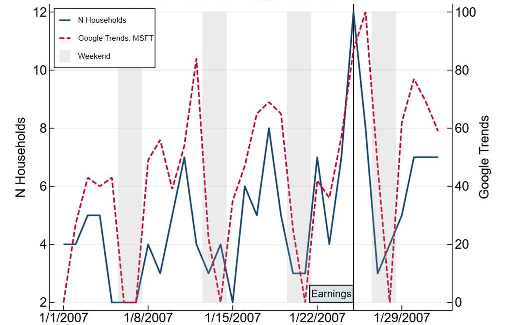
\includegraphics[width=\linewidth]{fig2a.pdf}\par 1/25 季度财报
    \column{.325\textwidth}\centering\small
     \textbf{B · Apple}\par
     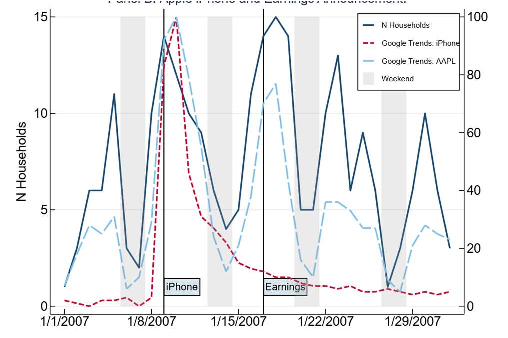
\includegraphics[width=\linewidth]{fig2b.pdf}\par 1/9 iPhone、1/17 财报
    \column{.325\textwidth}\centering\small
     \textbf{C · Sirius}\par
     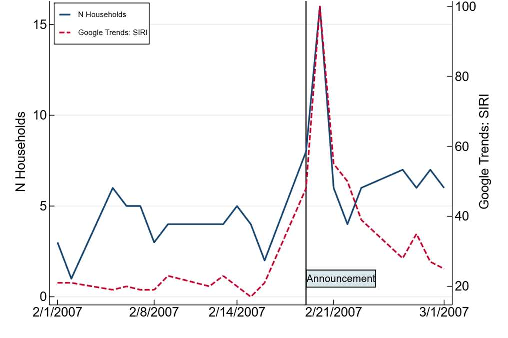
\includegraphics[width=\linewidth]{fig2c.pdf}\par 2/19 宣布与 XM 合并
  \end{columns}
  \medskip
  {\small\textcolor{sampleblue}{深蓝实线／左轴：每日研究人数}；\textcolor{wine}{红虚线／右轴：Google Trends}（MSFT、iPhone、SIRI）。}
  \finding{财报、新品与并购日期附近，点击流研究与搜索关注同时上升。}
\end{frame}

\begin{frame}[label=tilt]{股票特征对“看什么”的解释度较低}
  \crumb{Part 4}{4.1 股票与投资者 · 内容倾斜}{Table 4 (5)--(6)}
  {\small\textbf{被解释变量 \(D\)}＝看过价格类信息的投资者比例－看过基本面类信息的投资者比例。\par
  \scriptsize 价格类：价格图、技术；基本面类：盈利、股利、其他基本面、分析师、官网。}\par\smallskip
  \begin{columns}[T,onlytextwidth]
    \column{.61\textwidth}\small
    \textbf{价格覆盖率减基本面覆盖率，第 (6) 列}\par
    \begin{tikzpicture}[x=13cm,y=.52cm,font=\scriptsize]
      \draw[quiet!45] (0,-.33)--(0,3.44);
      \coefrow{3}{-.206}{.06}{4.63}{波动率}
      \coefrow{2}{-.206}{.05}{2.33}{动量}
      \coefrow{1}{-.206}{-.10}{-2.42}{分析师覆盖}
      \coefrow{0}{-.206}{.03}{.61}{市值（对数）}
      \foreach \x in {-.2,-.1,0,.1} \node[below] at (\x,-.34) {\pgfmathprintnumber{\x}};
    \end{tikzpicture}\par
    \column{.36\textwidth}\small
    \textbf{对照覆盖率规格}\par
    \greatnum{7.9\%}\par
    {\small 第 (5) 列 \(R^2\)}\par\smallskip
    {\large\bfseries\color{wine}9.0\%}\;第 (6) 列\par\smallskip
    同类扩展规格解释覆盖率时，\(R^2=48.4\%\)。
  \end{columns}
  \finding{股票特征只解释很少部分（8\%)的主题倾斜，说明高波动股票偏价格研究； 异质性的解释，需要继续对投资者考察。}
\end{frame}

